\documentclass[tikz, convert={outext=.png}]{standalone}

% use xelatex
\usepackage{fontspec}
\usepackage{pgffor}

\setmainfont{Ubuntu Mono}

\newcommand{\nullch}{\footnotesize{\textbackslash 0}}

\tikzstyle{arrgrid} = [rectangle, draw, minimum width = 0.5cm, minimum height = 0.5cm]

\begin{document}

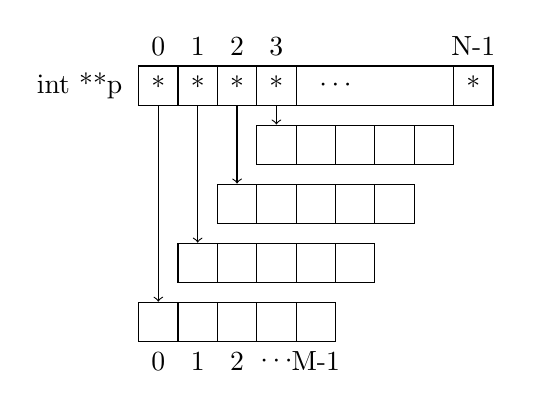
\begin{tikzpicture}
  \node at (-1, 0) {int **p};
  \foreach \i in {0, 1, 2, 3} {
    \node[arrgrid] (r\i) at (\i * 0.5, 0) {*};
    \node at (\i  * 0.5, 0.5) {\i};
  }
  \draw[-] (1.75, 0.25) -- (4, 0.25);
  \draw[-] (1.75, -0.25) -- (4, -0.25);
  \node[arrgrid] at (4, 0) {*};
  \node at (4, 0.5) {N-1};
  \node at (2.25, 0) {\(\cdots\)};
  \foreach \i in {0, 1, 2, 3} {
    \foreach \j in {0, 1, 2, 3, 4} {
      \node[arrgrid] (r\i\j) at (\i * 0.5 + \j * 0.5, -3 + 0.75 * \i) {};
    }
    \draw[->] (r\i) -- (r\i0);
  }
  \foreach \i\j in {0/0, 1/1, 2/2, 3/{\(\cdots\)}, 4/{M-1}} {
    \node at (\i * 0.5, -3.5) {\j};
  }
\end{tikzpicture}

\end{document}